\documentclass{sig-alternate-05-2015}
\usepackage{hyperref}


\begin{document}

% Copyright
%\setcopyright{acmcopyright}
% DOI
\doi{insert doi here}

% ISBN
\isbn{insert isbn here}

\title{BigBInf Micro Cloud Platform}

\numberofauthors{1}
\author{
% 1st. author
\alignauthor
Brendan D. Ball\\
       \affaddr{University of Cape Town}\\
}

\date{30 August 2015}


\maketitle
\begin{abstract}
[Abstract]
\end{abstract}
\keywords{Big Data; BioInformatics; Clouds}


\section{Background}
Cloud infrastructure would go a long way in simplifying the processing of big data. Collaboration between researchers can potentially improve if they are able to process the same raw data while being in different locations. This would be done by keeping the data in a cloud solution and allowing researchers access to execute code on the raw data. There has been an explorative push towards cloud solutions from Amazon, Google etc, but there are significant drawbacks. The raw data needs to be uploaded initially and researchers often resort to mailing hard drives \cite{baker2010next}. 
\\
\\
An example of progress towards a cloud solution specifically for bioinformatics is Cloud BioLinux, which is a community driven project focussed on next generation sequencing. It is a toolkit which makes it easy to deploy virtual machines with bioinformatics infrastructure to a cloud platform. It bundles specific packages used in next generation sequence analysis, thereby decreasing configuration time and increasing maintainability. Instances of Cloud BioLinux have been tested on the Amazon EC2 cloud platform and on a private Eucalyptus cloud \cite{krampis2012cloud}.
\\
\\
Micro clouds deployed on-site would overcome the challenge of uploading big data to a commercial cloud. However, since different research institutions would deploy their own micro clouds, a need for cloud interoperability arises to maintain the ability for researchers from different institutions to collaborate on the same data. The cloud interoperability will form a community cloud. A use case of a specific community cloud has some similar architectural properties to what we are looking for. These properties include autonomy (where each micro cloud will be managed independently), security, self management of nodes, and scalable \cite{jimenez2014deploying}.
\\
\\
The traditional approach to creating a cloud platform which allows users to run their own instances of operating systems (such as Amazon EC2) is using virtualisation technology. This includes both hardware level emulation support and the software needed to manage the virtualisation. These virtualisation schemes use machine level virtualisation \cite{fink2014docker}. A new method, known as containerization provides much of the same functionality with added benefits of lower resource usage and better performance. Containers are able to run native machine instructions compared to virtualisation emulating every machine instruction \cite{dua2014virtualization}. Of course this means that containers are only useful when complete virtualisation is not needed, instead containers allow isolated application deployment and portability.

\section{Design}
This project is a collaboration between UCT and UWC. We met with the supervisors at UWC and continued communication with feedback was ongoing throughout the project lifetime. UCT E-Research was subsequently also brought onboard the project. Both UWC and UCT E-Research provided valuable hardware resources enabling thorough evaluation in a real world setting.

\subsection{Design Aims}
The main problem that this project is trying to solve is processing of Big Data. This means that we have to be able to access the data that sits on the micro cloud. This project aims to address this problem by allowing code to be uploaded by a user and executed on local data. Users will do this by interacting with a front end web interface. The functionality of the platform is of primary concern, thus user interface design will not be considered and is outside the scope of this project. 
\\\\
As multiple jobs can be submitted by multiple people, these jobs have to be scheduled properly to allow successful completion of each job. The whole platform should be fairly modular to allow pluggable components. This will allow possibilities such as adding a different scheduler or completely replacing the backend while keeping the front end web interface.
\\\\
The final aim is to form a community cloud. The community cloud will allow sharing of data and collaboration of users between multiple micro clouds.

\subsection{Constraints}
Micro cloud deployments for evaluation are limited to UWC and UCT E-Research. This means that the community cloud that will be evaluated will only consist of two micro clouds.

\subsection{Approach}
\begin{figure}
\centering
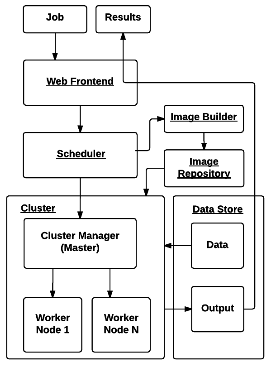
\includegraphics[scale=0.8]{img/microcloud_architecture}
\caption{Micro Cloud Architecture}
\end{figure}
\subsubsection{Jobs}
This project's source code will be stored in a version control system (VCS). Software also needs to be verified for correctness to decrease the chance of bugs occurring. This will be done by writing unit tests to allow continuous testing at all stages of the project.

\subsubsection{Micro Cloud Components}
The platform will consist of a few different components including, a web interface, a scheduler, a cluster manager (the master node), multiple worker nodes, and finally a storage interface which will allow reading from and writing to persistent storage. 



\subsection{Evaluation}
The functionality of the micro cloud will be evaluated by submitting sample analysis code as a job. The analysis code will be searching against a genome database from NCBI's NR database which is publicly available. The analysis code will make use of the BLAST+ search tool. The code itself will be custom queries. Different sized jobs can be tested by increasing or decreasing the size of the query which makes it easily scalable to have different sized test cases.



\subsection{Implementation}


A job describes a single instance of code being uploaded to be executed. 
The micro cloud platform will make use of containers, more specifically Docker containers to execute code. Docker images are created using Dockerfiles which specify the execution environment and what files to execute. This means that submitting a job will require creating a Dockerfile and uploading this along with source code which will be executed. 

\subsubsection{Cluster Manager - Kubernetes}
In this project cluster manager is synonomous with container manager because the cluster will strictly operate by running containers. Kubernetes has been chosen as the cluster manager framework for managing the micro cloud. Kubernetes is specifically designed to run docker containers in a cluster. It is still a new system and Kubernetes version 1 has just recently been released which means it's ready for production use. Using containers instead of virtual machines has only recently become popular. The growth in popularity has resulted in a number of systems being developed which provide some overlapping functionality to Kubernetes. Kubernetes looks most promising as it is easy to use. Given that it is relatively new it is not cluttered and aims to solve a single problem of being a container manager. 

\subsubsection{OpenStack}
OpenStack was the first system looked at as a base for a container manager. After much trouble trying to get it set up properly in a development environment it was decided that there are more suitable systems to solve the problem. OpenStack is very cluttered with many inter dependent components. The OpenStack Swift API will however be supported for storage as it is very likely that the micro cloud platform could be deployed on top of OpenStack.


\subsubsection{Scheduler}
The default scheduler will rely on a first-in-first-out (FIFO) queue to schedule jobs.

\subsubsection{Storage}
The two most popular storage APIs are OpenStack Swift API and S3 API. By supporting both of these storage APIs it should be relatively easy to deploy the micro cloud on a large range of different clusters.

\subsubsection{Web Interface}
The backend web interface will be implemented using the python flask web framework. It is a minimalist framework which allows for rapid development of web interfaces. 
The front end web interface will be implemented using Angularjs to create a single page application. 
draw
\subsubsection{Community Cloud}
A community cloud will be formed by implementing a centralised discovery service. This will improve scalability compared to a full mesh network between micro clouds.

\subsubsection{VCS}
Git will be used as the version control system for storing all the source code for the micro cloud platform.


\bibliographystyle{ACM-Reference-Format-Journals}
\bibliography{ref} 


\end{document}
